\chapter{Preliminares}
Funciones.\index{funciones}


- DENOTAR CRITERIOS DE CONGRUENCIA COMO \textbf{cc(???)}

\section{Área de objetos en el plano.}
En esta sección nos daremos a la tarea de contestar la siguiente pregunta: ¿Cómo calcular el área de objetos en el plano? Es probable que nos venga a la mente alguna fórmula que conocemos desde la educación básica para el cálculo de áreas, pero buscaremos una manera de deducir dichas expresiones.

Para comenzar, daremos la siguiente definición:

\begin{df}\label{paralelogramo}
Sea $\{A, B, C, D\}$ un conjunto de puntos distintos en el plano, no colineales de tres en tres. Decimos que  el conjunto $\{A, B, C, D\}$ es un \textcolor{red}{\bf paralelogramo}\index{paralelogramo}, que denotaremos como $\square ABCD$, si y solamente si se cumplen las siguientes condiciones:
\begin{itemize}
\item $\overline{AB}$ es paralela a $\overline{CD}$
\item $\overline{CB}$ es paralela a $\overline{DA}$
\end{itemize}
\end{df}

Como consecuencia de esto, daremos otras definiciones:

\begin{df}.
\begin{itemize}
\item Un paralelogramo $\square ABCD$ es un \textcolor{red}{\textbf{rectángulo}}\index{rectángulo} si y solamente si $\square ABCD$ es un paralelogramo con un ángulo interno recto.
\item Un paralelogramo $\square ABCD$ es un \textcolor{red}{{\bf cuadrado}}\index{cuadrado} si y solamente si $\square ABCD$ es un rectángulo en el que $|AB|=|BC|=|CD|=|DA|$.
\end{itemize}
\end{df}

El \index{área}área de un objeto es una medida que asignamos a dicho objeto. Por ejemplo, otras medidas que se pueden establecer entre los objetos son la longitud, el peso, la temperatura, etcétera. \\

Ahora, ¿cómo determinamos las diferentes medidas de los diferentes objetos?

Toda medida requiere de una unidad de medida para compararla; por ejemplo:
\begin{itemize}
\item Para determinar la longitud de un objeto se tiene que calcular cuántas veces la unidad llamada \textit{metro} es necesaria para tener la longitud del mismo.

\item Para calcular el peso de un objeto, se debe calcular cuántas veces la unidad de medida llamada \textit{gramo} es necesaria para tener el peso del mismo.
\end{itemize}

Así, para calcular el área de un objeto, necesitamos tener una unidad de medida que nos permita calcularla.

\begin{df}
Definiremos \index{unidad cuadrada} \textcolor{red}{{\bf unidad cuadrada}} al cuadrado que por lado mide una unidad. Es decir, una unidad cuadrada es la cantidad de espacio del plano, contenidad en un cuadrado $\square ABCD$ tal que $|AB|=1$.

\begin{figure}[!h]
\begin{center}
\definecolor{zzttqq}{rgb}{0.6,0.2,0.}
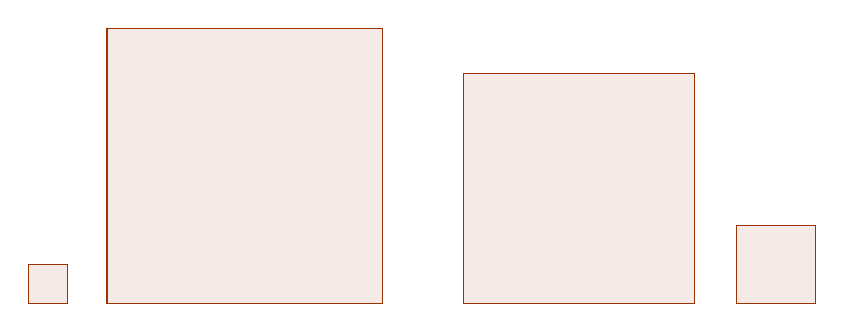
\begin{tikzpicture}[x=0.5cm,y=0.5cm]
\fill[color=zzttqq,fill=zzttqq,fill opacity=0.1] (1.06,0.) -- (6.92,0.) -- (6.92,5.86) -- (1.06,5.86) -- cycle;
\fill[color=zzttqq,fill=zzttqq,fill opacity=0.1] (8.,0.) -- (10.,0.) -- (10.,2.) -- (8.,2.) -- cycle;
\fill[color=zzttqq,fill=zzttqq,fill opacity=0.1] (-8.,0.) -- (-1.,0.) -- (-1.,7.) -- (-8.,7.) -- cycle;
\fill[color=zzttqq,fill=zzttqq,fill opacity=0.1] (-10.,0.) -- (-9.,0.) -- (-9.,1.) -- (-10.,1.) -- cycle;
\draw [color=zzttqq] (1.06,0.)-- (6.92,0.);
\draw [color=zzttqq] (6.92,0.)-- (6.92,5.86);
\draw [color=zzttqq] (6.92,5.86)-- (1.06,5.86);
\draw [color=zzttqq] (1.06,5.86)-- (1.06,0.);
\draw [color=zzttqq] (8.,0.)-- (10.,0.);
\draw [color=zzttqq] (10.,0.)-- (10.,2.);
\draw [color=zzttqq] (10.,2.)-- (8.,2.);
\draw [color=zzttqq] (8.,2.)-- (8.,0.);
\draw [color=zzttqq] (-8.,0.)-- (-1.,0.);
\draw [color=zzttqq] (-1.,0.)-- (-1.,7.);
\draw [color=zzttqq] (-1.,7.)-- (-8.,7.);
\draw [color=zzttqq] (-8.,7.)-- (-8.,0.);
\draw [color=zzttqq] (-10.,0.)-- (-9.,0.);
\draw [color=zzttqq] (-9.,0.)-- (-9.,1.);
\draw [color=zzttqq] (-9.,1.)-- (-10.,1.);
\draw [color=zzttqq] (-10.,1.)-- (-10.,0.);
\end{tikzpicture}
\caption{Diferentes unidades cuadradas.}\label{unidadcuadrada}
\end{center}
\end{figure}
\end{df}

\begin{df}\label{dfárea}\index{área}
Sea $P$ un subconjunto del plano. $\alpha$ es el \textcolor{red}{\textbf{área}} de $P$ si y solamente sí caben $\alpha$ unidades cuadradas dentro de $P$. Al área la denotaremos como $\alpha = \A(P)$.
\end{df}

Con esta convención, veamos cómo calcular áreas de objetos planos.

\begin{ej}
¿Qué área tiene un cuadrado cuyos lados miden $\frac{9}{8}$ unidades?
\end{ej}
\begin{pba}

%%%%%%%%%
%%%%%%%%%
%%%%%%%%%

Primero veamos la figura~\ref{cuadrado97}, en donde representaremos un cuadrado cuyos lados miden $\frac {17}{16}$ unidades.

\begin{figure}[!h]
\begin{center}
\definecolor{ffqqqq}{rgb}{1.,0.,0.}
\definecolor{zzttqq}{rgb}{0.6,0.2,0.}
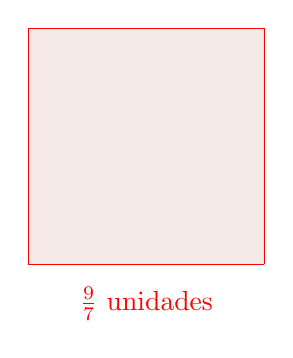
\begin{tikzpicture}[x=0.5cm,y=0.5cm]
\fill[color=zzttqq,fill=zzttqq,fill opacity=0.1] (-3,0) -- (3,0) -- (3,6) -- (-3,6) -- cycle;
\draw [color=ffqqqq] (-3,0) -- (3,0);
\draw [color=ffqqqq] (3,0) -- (3,6);
\draw [color=ffqqqq] (3,6) -- (-3,6);
\draw [color=ffqqqq] (-3,6) -- (-3,0);
\draw[color=ffqqqq] (0,-1) node {$\frac{9}{7}$ \text{unidades}};
\end{tikzpicture}
\caption{Cuadrado de lado $\frac{9}{7}$ unidades.}\label{cuadrado97}
\end{center}
\end{figure}

Para calcular el área del cuadrado, debemos determinar de cuántas unidades cuadradas está formado, es decir, calcular la cantidad de cuadrados (cuyo lado mide una unidad) que caben en un cuadrado. Dado que el cuadrado tiene por lado $\frac{9}{7}$ unidades, determinemos unidades en una de sus bases para construir cuadrados que midan por lado una unidad, como en la figura~\ref{cuadradocuadrado}. \\

\begin{figure}[!h]
\begin{center}
\definecolor{ffqqqq}{rgb}{1.,0.,0.}
\definecolor{zzttqq}{rgb}{0.6,0.2,0.}
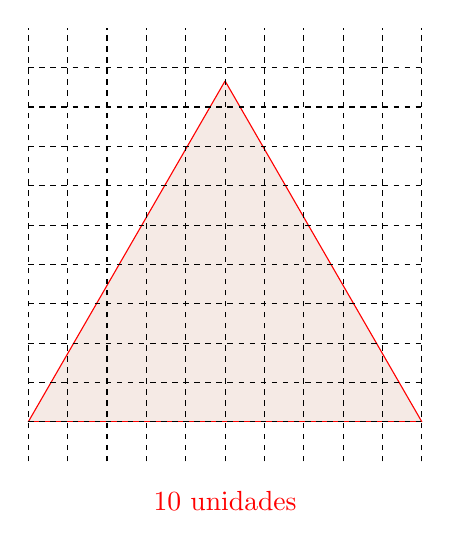
\begin{tikzpicture}[x=0.5cm,y=0.5cm]
\fill[color=zzttqq,fill=zzttqq,fill opacity=0.1] (-5.,0.) -- (5.,0.) -- (0.,8.66025403784) -- cycle;
\draw [color=ffqqqq] (-5.,0.)-- (5.,0.);
\draw [color=ffqqqq] (5.,0.)-- (0.,8.66025403784);
\draw [color=ffqqqq] (0.,8.66025403784)-- (-5.,0.);

\draw [dash pattern=on 2pt off 2pt] (-5,-1) -- (-5,10);
\draw [dash pattern=on 2pt off 2pt] (-4,-1) -- (-4,10);
\draw [dash pattern=on 2pt off 2pt] (-3,-1) -- (-3,10);
\draw [dash pattern=on 2pt off 2pt] (-2,-1) -- (-2,10);
\draw [dash pattern=on 2pt off 2pt] (-1,-1) -- (-1,10);
\draw [dash pattern=on 2pt off 2pt] (0,-1) -- (0,10);
\draw [dash pattern=on 2pt off 2pt] (1,-1) -- (1,10);
\draw [dash pattern=on 2pt off 2pt] (2,-1) -- (2,10);
\draw [dash pattern=on 2pt off 2pt] (3,-1) -- (3,10);
\draw [dash pattern=on 2pt off 2pt] (4,-1) -- (4,10);
\draw [dash pattern=on 2pt off 2pt] (5,-1) -- (5,10);

\draw [dash pattern=on 2pt off 2pt] (-5,0) -- (5,0);
\draw [dash pattern=on 2pt off 2pt] (-5,1) -- (5,1);
\draw [dash pattern=on 2pt off 2pt] (-5,2) -- (5,2);
\draw [dash pattern=on 2pt off 2pt] (-5,3) -- (5,3);
\draw [dash pattern=on 2pt off 2pt] (-5,4) -- (5,4);
\draw [dash pattern=on 2pt off 2pt] (-5,5) -- (5,5);
\draw [dash pattern=on 2pt off 2pt] (-5,6) -- (5,6);
\draw [dash pattern=on 2pt off 2pt] (-5,7) -- (5,7);
\draw [dash pattern=on 2pt off 2pt] (-5,8) -- (5,8);
\draw [dash pattern=on 2pt off 2pt] (-5,9) -- (5,9);
\draw [dash pattern=on 2pt off 2pt] (5,-1) -- (5,10);

\draw[color=ffqqqq] (0,-2) node {\text{10 unidades}};
\end{tikzpicture}
\caption{Triángulo equilátero cuyo lado mide 10 unidades.}\label{cuadradocuadrado}
\end{center}
\end{figure}

Al contar la cantidad de unidades cuadradas que están contenidas en el triángulo, tenemos que solamente hay 30 (figura~\ref{triangulounidaddentro}). \\

\begin{figure}[!h]
\begin{center}
\definecolor{ffqqqq}{rgb}{1.,0.,0.}
\definecolor{zzttqq}{rgb}{0.6,0.2,0.}
\definecolor{qqqqff}{rgb}{0.,0.,1.}
\definecolor{ffqqqq}{rgb}{1.,0.,0.}
\definecolor{zzttqq}{rgb}{0.6,0.2,0.}
\definecolor{cqcqcq}{rgb}{0.752941176471,0.752941176471,0.752941176471}

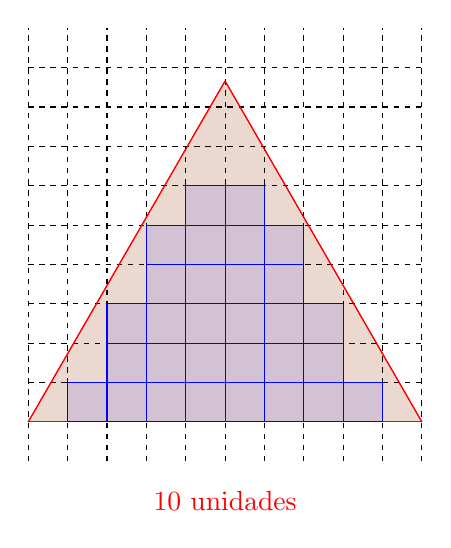
\begin{tikzpicture}[x=0.5cm,y=0.5cm]
\fill[color=zzttqq,fill=zzttqq,fill opacity=0.1] (-5.,0.) -- (5.,0.) -- (0.,8.66025403784) -- cycle;
\draw [color=ffqqqq] (-5.,0.)-- (5.,0.);
\draw [color=ffqqqq] (5.,0.)-- (0.,8.66025403784);
\draw [color=ffqqqq] (0.,8.66025403784)-- (-5.,0.);

\draw [dash pattern=on 2pt off 2pt] (-5,-1) -- (-5,10);
\draw [dash pattern=on 2pt off 2pt] (-4,-1) -- (-4,10);
\draw [dash pattern=on 2pt off 2pt] (-3,-1) -- (-3,10);
\draw [dash pattern=on 2pt off 2pt] (-2,-1) -- (-2,10);
\draw [dash pattern=on 2pt off 2pt] (-1,-1) -- (-1,10);
\draw [dash pattern=on 2pt off 2pt] (0,-1) -- (0,10);
\draw [dash pattern=on 2pt off 2pt] (1,-1) -- (1,10);
\draw [dash pattern=on 2pt off 2pt] (2,-1) -- (2,10);
\draw [dash pattern=on 2pt off 2pt] (3,-1) -- (3,10);
\draw [dash pattern=on 2pt off 2pt] (4,-1) -- (4,10);
\draw [dash pattern=on 2pt off 2pt] (5,-1) -- (5,10);

\draw [dash pattern=on 2pt off 2pt] (-5,0) -- (5,0);
\draw [dash pattern=on 2pt off 2pt] (-5,1) -- (5,1);
\draw [dash pattern=on 2pt off 2pt] (-5,2) -- (5,2);
\draw [dash pattern=on 2pt off 2pt] (-5,3) -- (5,3);
\draw [dash pattern=on 2pt off 2pt] (-5,4) -- (5,4);
\draw [dash pattern=on 2pt off 2pt] (-5,5) -- (5,5);
\draw [dash pattern=on 2pt off 2pt] (-5,6) -- (5,6);
\draw [dash pattern=on 2pt off 2pt] (-5,7) -- (5,7);
\draw [dash pattern=on 2pt off 2pt] (-5,8) -- (5,8);
\draw [dash pattern=on 2pt off 2pt] (-5,9) -- (5,9);
\draw [dash pattern=on 2pt off 2pt] (5,-1) -- (5,10);


\fill[color=zzttqq,fill=zzttqq,fill opacity=0.1] (-5.,0.) -- (5.,0.) -- (0.,8.66025403784) -- cycle;
\fill[color=qqqqff,fill=qqqqff,fill opacity=0.1] (-4.,0.) -- (-3.,0.) -- (-3.,1.) -- (-4.,1.) -- cycle;
\fill[color=qqqqff,fill=qqqqff,fill opacity=0.1] (-3.,0.) -- (-2.,0.) -- (-2.,1.) -- (-3.,1.) -- cycle;
\fill[color=qqqqff,fill=qqqqff,fill opacity=0.1] (-3.,1.) -- (-2.,1.) -- (-2.,2.) -- (-3.,2.) -- cycle;
\fill[color=qqqqff,fill=qqqqff,fill opacity=0.1] (-3.,2.) -- (-2.,2.) -- (-2.,3.) -- (-3.,3.) -- cycle;
\fill[color=qqqqff,fill=qqqqff,fill opacity=0.1] (-2.,3.) -- (-1.,3.) -- (-1.,4.) -- (-2.,4.) -- cycle;
\fill[color=qqqqff,fill=qqqqff,fill opacity=0.1] (-2.,4.) -- (-1.,4.) -- (-1.,5.) -- (-2.,5.) -- cycle;
\fill[color=qqqqff,fill=qqqqff,fill opacity=0.1] (-1.,5.) -- (0.,5.) -- (0.,6.) -- (-1.,6.) -- cycle;
\fill[color=qqqqff,fill=qqqqff,fill opacity=0.1] (0.,5.) -- (1.,5.) -- (1.,6.) -- (0.,6.) -- cycle;
\fill[color=qqqqff,fill=qqqqff,fill opacity=0.1] (0.,4.) -- (1.,4.) -- (1.,5.) -- (0.,5.) -- cycle;
\fill[color=qqqqff,fill=qqqqff,fill opacity=0.1] (-1.,4.) -- (0.,4.) -- (0.,5.) -- (-1.,5.) -- cycle;
\fill[color=qqqqff,fill=qqqqff,fill opacity=0.1] (1.,4.) -- (2.,4.) -- (2.,5.) -- (1.,5.) -- cycle;
\fill[color=qqqqff,fill=qqqqff,fill opacity=0.1] (1.,3.) -- (2.,3.) -- (2.,4.) -- (1.,4.) -- cycle;
\fill[color=qqqqff,fill=qqqqff,fill opacity=0.1] (2.,2.) -- (3.,2.) -- (3.,3.) -- (2.,3.) -- cycle;
\fill[color=qqqqff,fill=qqqqff,fill opacity=0.1] (3.,0.) -- (4.,0.) -- (4.,1.) -- (3.,1.) -- cycle;
\fill[color=qqqqff,fill=qqqqff,fill opacity=0.1] (2.,1.) -- (3.,1.) -- (3.,2.) -- (2.,2.) -- cycle;
\fill[color=qqqqff,fill=qqqqff,fill opacity=0.1] (2.,0.) -- (3.,0.) -- (3.,1.) -- (2.,1.) -- cycle;
\fill[color=qqqqff,fill=qqqqff,fill opacity=0.1] (0.,3.) -- (1.,3.) -- (1.,4.) -- (0.,4.) -- cycle;
\fill[color=qqqqff,fill=qqqqff,fill opacity=0.1] (-1.,3.) -- (0.,3.) -- (0.,4.) -- (-1.,4.) -- cycle;
\fill[color=qqqqff,fill=qqqqff,fill opacity=0.1] (-2.,2.) -- (-1.,2.) -- (-1.,3.) -- (-2.,3.) -- cycle;
\fill[color=qqqqff,fill=qqqqff,fill opacity=0.1] (-1.,2.) -- (0.,2.) -- (0.,3.) -- (-1.,3.) -- cycle;
\fill[color=qqqqff,fill=qqqqff,fill opacity=0.1] (0.,2.) -- (1.,2.) -- (1.,3.) -- (0.,3.) -- cycle;
\fill[color=qqqqff,fill=qqqqff,fill opacity=0.1] (1.,2.) -- (2.,2.) -- (2.,3.) -- (1.,3.) -- cycle;
\fill[color=qqqqff,fill=qqqqff,fill opacity=0.1] (-2.,1.) -- (-1.,1.) -- (-1.,2.) -- (-2.,2.) -- cycle;
\fill[color=qqqqff,fill=qqqqff,fill opacity=0.1] (-1.,1.) -- (0.,1.) -- (0.,2.) -- (-1.,2.) -- cycle;
\fill[color=qqqqff,fill=qqqqff,fill opacity=0.1] (0.,1.) -- (1.,1.) -- (1.,2.) -- (0.,2.) -- cycle;
\fill[color=qqqqff,fill=qqqqff,fill opacity=0.1] (1.,1.) -- (2.,1.) -- (2.,2.) -- (1.,2.) -- cycle;
\fill[color=qqqqff,fill=qqqqff,fill opacity=0.1] (-2.,0.) -- (-1.,0.) -- (-1.,1.) -- (-2.,1.) -- cycle;
\fill[color=qqqqff,fill=qqqqff,fill opacity=0.1] (-1.,0.) -- (0.,0.) -- (0.,1.) -- (-1.,1.) -- cycle;
\fill[color=qqqqff,fill=qqqqff,fill opacity=0.1] (0.,0.) -- (1.,0.) -- (1.,1.) -- (0.,1.) -- cycle;
\fill[color=qqqqff,fill=qqqqff,fill opacity=0.1] (1.,0.) -- (2.,0.) -- (2.,1.) -- (1.,1.) -- cycle;
\draw [color=ffqqqq] (-5.,0.)-- (5.,0.);
\draw [color=ffqqqq] (5.,0.)-- (0.,8.66025403784);
\draw [color=ffqqqq] (0.,8.66025403784)-- (-5.,0.);
\draw [color=qqqqff] (-4.,0.)-- (-3.,0.);
\draw [color=qqqqff] (-3.,0.)-- (-3.,1.);
\draw [color=qqqqff] (-3.,1.)-- (-4.,1.);
\draw [color=qqqqff] (-4.,1.)-- (-4.,0.);
\draw [color=qqqqff] (-3.,0.)-- (-2.,0.);
\draw [color=qqqqff] (-2.,0.)-- (-2.,1.);
\draw [color=qqqqff] (-2.,1.)-- (-3.,1.);
\draw [color=qqqqff] (-3.,1.)-- (-3.,0.);
\draw [color=qqqqff] (-3.,1.)-- (-2.,1.);
\draw [color=qqqqff] (-2.,1.)-- (-2.,2.);
\draw [color=qqqqff] (-2.,2.)-- (-3.,2.);
\draw [color=qqqqff] (-3.,2.)-- (-3.,1.);
\draw [color=qqqqff] (-3.,2.)-- (-2.,2.);
\draw [color=qqqqff] (-2.,2.)-- (-2.,3.);
\draw [color=qqqqff] (-2.,3.)-- (-3.,3.);
\draw [color=qqqqff] (-3.,3.)-- (-3.,2.);
\draw [color=qqqqff] (-2.,3.)-- (-1.,3.);
\draw [color=qqqqff] (-1.,3.)-- (-1.,4.);
\draw [color=qqqqff] (-1.,4.)-- (-2.,4.);
\draw [color=qqqqff] (-2.,4.)-- (-2.,3.);
\draw [color=qqqqff] (-2.,4.)-- (-1.,4.);
\draw [color=qqqqff] (-1.,4.)-- (-1.,5.);
\draw [color=qqqqff] (-1.,5.)-- (-2.,5.);
\draw [color=qqqqff] (-2.,5.)-- (-2.,4.);
\draw [color=qqqqff] (-1.,5.)-- (0.,5.);
\draw [color=qqqqff] (0.,5.)-- (0.,6.);
\draw [color=qqqqff] (0.,6.)-- (-1.,6.);
\draw [color=qqqqff] (-1.,6.)-- (-1.,5.);
\draw [color=qqqqff] (0.,5.)-- (1.,5.);
\draw [color=qqqqff] (1.,5.)-- (1.,6.);
\draw [color=qqqqff] (1.,6.)-- (0.,6.);
\draw [color=qqqqff] (0.,6.)-- (0.,5.);
\draw [color=qqqqff] (0.,4.)-- (1.,4.);
\draw [color=qqqqff] (1.,4.)-- (1.,5.);
\draw [color=qqqqff] (1.,5.)-- (0.,5.);
\draw [color=qqqqff] (0.,5.)-- (0.,4.);
\draw [color=qqqqff] (-1.,4.)-- (0.,4.);
\draw [color=qqqqff] (0.,4.)-- (0.,5.);
\draw [color=qqqqff] (0.,5.)-- (-1.,5.);
\draw [color=qqqqff] (-1.,5.)-- (-1.,4.);
\draw [color=qqqqff] (1.,4.)-- (2.,4.);
\draw [color=qqqqff] (2.,4.)-- (2.,5.);
\draw [color=qqqqff] (2.,5.)-- (1.,5.);
\draw [color=qqqqff] (1.,5.)-- (1.,4.);
\draw [color=qqqqff] (1.,3.)-- (2.,3.);
\draw [color=qqqqff] (2.,3.)-- (2.,4.);
\draw [color=qqqqff] (2.,4.)-- (1.,4.);
\draw [color=qqqqff] (1.,4.)-- (1.,3.);
\draw [color=qqqqff] (2.,2.)-- (3.,2.);
\draw [color=qqqqff] (3.,2.)-- (3.,3.);
\draw [color=qqqqff] (3.,3.)-- (2.,3.);
\draw [color=qqqqff] (2.,3.)-- (2.,2.);
\draw [color=qqqqff] (3.,0.)-- (4.,0.);
\draw [color=qqqqff] (4.,0.)-- (4.,1.);
\draw [color=qqqqff] (4.,1.)-- (3.,1.);
\draw [color=qqqqff] (3.,1.)-- (3.,0.);
\draw [color=qqqqff] (2.,1.)-- (3.,1.);
\draw [color=qqqqff] (3.,1.)-- (3.,2.);
\draw [color=qqqqff] (3.,2.)-- (2.,2.);
\draw [color=qqqqff] (2.,2.)-- (2.,1.);
\draw [color=qqqqff] (2.,0.)-- (3.,0.);
\draw [color=qqqqff] (3.,0.)-- (3.,1.);
\draw [color=qqqqff] (3.,1.)-- (2.,1.);
\draw [color=qqqqff] (2.,1.)-- (2.,0.);
\draw [color=qqqqff] (0.,3.)-- (1.,3.);
\draw [color=qqqqff] (1.,3.)-- (1.,4.);
\draw [color=qqqqff] (1.,4.)-- (0.,4.);
\draw [color=qqqqff] (0.,4.)-- (0.,3.);
\draw [color=qqqqff] (-1.,3.)-- (0.,3.);
\draw [color=qqqqff] (0.,3.)-- (0.,4.);
\draw [color=qqqqff] (0.,4.)-- (-1.,4.);
\draw [color=qqqqff] (-1.,4.)-- (-1.,3.);
\draw [color=qqqqff] (-2.,2.)-- (-1.,2.);
\draw [color=qqqqff] (-1.,2.)-- (-1.,3.);
\draw [color=qqqqff] (-1.,3.)-- (-2.,3.);
\draw [color=qqqqff] (-2.,3.)-- (-2.,2.);
\draw [color=qqqqff] (-1.,2.)-- (0.,2.);
\draw [color=qqqqff] (0.,2.)-- (0.,3.);
\draw [color=qqqqff] (0.,3.)-- (-1.,3.);
\draw [color=qqqqff] (-1.,3.)-- (-1.,2.);
\draw [color=qqqqff] (0.,2.)-- (1.,2.);
\draw [color=qqqqff] (1.,2.)-- (1.,3.);
\draw [color=qqqqff] (1.,3.)-- (0.,3.);
\draw [color=qqqqff] (0.,3.)-- (0.,2.);
\draw [color=qqqqff] (1.,2.)-- (2.,2.);
\draw [color=qqqqff] (2.,2.)-- (2.,3.);
\draw [color=qqqqff] (2.,3.)-- (1.,3.);
\draw [color=qqqqff] (1.,3.)-- (1.,2.);
\draw [color=qqqqff] (-2.,1.)-- (-1.,1.);
\draw [color=qqqqff] (-1.,1.)-- (-1.,2.);
\draw [color=qqqqff] (-1.,2.)-- (-2.,2.);
\draw [color=qqqqff] (-2.,2.)-- (-2.,1.);
\draw [color=qqqqff] (-1.,1.)-- (0.,1.);
\draw [color=qqqqff] (0.,1.)-- (0.,2.);
\draw [color=qqqqff] (0.,2.)-- (-1.,2.);
\draw [color=qqqqff] (-1.,2.)-- (-1.,1.);
\draw [color=qqqqff] (0.,1.)-- (1.,1.);
\draw [color=qqqqff] (1.,1.)-- (1.,2.);
\draw [color=qqqqff] (1.,2.)-- (0.,2.);
\draw [color=qqqqff] (0.,2.)-- (0.,1.);
\draw [color=qqqqff] (1.,1.)-- (2.,1.);
\draw [color=qqqqff] (2.,1.)-- (2.,2.);
\draw [color=qqqqff] (2.,2.)-- (1.,2.);
\draw [color=qqqqff] (1.,2.)-- (1.,1.);
\draw [color=qqqqff] (-2.,0.)-- (-1.,0.);
\draw [color=qqqqff] (-1.,0.)-- (-1.,1.);
\draw [color=qqqqff] (-1.,1.)-- (-2.,1.);
\draw [color=qqqqff] (-2.,1.)-- (-2.,0.);
\draw [color=qqqqff] (-1.,0.)-- (0.,0.);
\draw [color=qqqqff] (0.,0.)-- (0.,1.);
\draw [color=qqqqff] (0.,1.)-- (-1.,1.);
\draw [color=qqqqff] (-1.,1.)-- (-1.,0.);
\draw [color=qqqqff] (0.,0.)-- (1.,0.);
\draw [color=qqqqff] (1.,0.)-- (1.,1.);
\draw [color=qqqqff] (1.,1.)-- (0.,1.);
\draw [color=qqqqff] (0.,1.)-- (0.,0.);
\draw [color=qqqqff] (1.,0.)-- (2.,0.);
\draw [color=qqqqff] (2.,0.)-- (2.,1.);
\draw [color=qqqqff] (2.,1.)-- (1.,1.);
\draw [color=qqqqff] (1.,1.)-- (1.,0.);

\draw[color=ffqqqq] (0,-2) node {\text{10 unidades}};
\end{tikzpicture}
\caption{Unidades cuadradas contenidas en el triángulo.}\label{triangulounidaddentro}
\end{center}
\end{figure}
 
También, podemos aproximarnos al área del triángulo al contar la cantidad de unidades cuadradas que contienen al triángulo; tenemos que solamente hay 58 unidades cuadradas (figura~\ref{triangulounidadfuera}).

\newpage

\begin{figure}[!h]
\begin{center}
\definecolor{ffqqqq}{rgb}{1.,0.,0.}
\definecolor{zzttqq}{rgb}{0.6,0.2,0.}
\definecolor{qqqqff}{rgb}{0.,0.,1.}
\definecolor{ffqqqq}{rgb}{1.,0.,0.}
\definecolor{zzttqq}{rgb}{0.6,0.2,0.}
\definecolor{cqcqcq}{rgb}{0.752941176471,0.752941176471,0.752941176471}

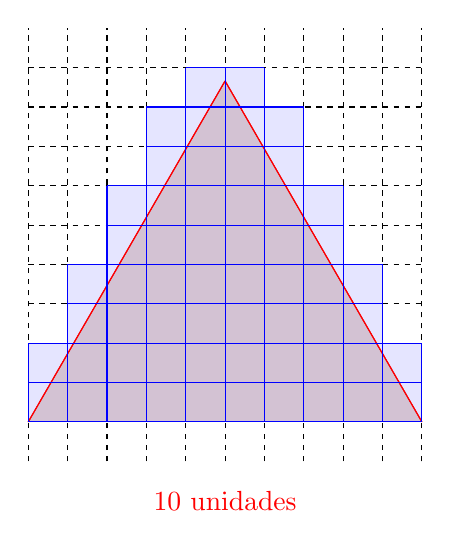
\begin{tikzpicture}[x=0.5cm,y=0.5cm]
\fill[color=zzttqq,fill=zzttqq,fill opacity=0.1] (-5.,0.) -- (5.,0.) -- (0.,8.66025403784) -- cycle;
\draw [color=ffqqqq] (-5.,0.)-- (5.,0.);
\draw [color=ffqqqq] (5.,0.)-- (0.,8.66025403784);
\draw [color=ffqqqq] (0.,8.66025403784)-- (-5.,0.);

\draw [dash pattern=on 2pt off 2pt] (-5,-1) -- (-5,10);
\draw [dash pattern=on 2pt off 2pt] (-4,-1) -- (-4,10);
\draw [dash pattern=on 2pt off 2pt] (-3,-1) -- (-3,10);
\draw [dash pattern=on 2pt off 2pt] (-2,-1) -- (-2,10);
\draw [dash pattern=on 2pt off 2pt] (-1,-1) -- (-1,10);
\draw [dash pattern=on 2pt off 2pt] (0,-1) -- (0,10);
\draw [dash pattern=on 2pt off 2pt] (1,-1) -- (1,10);
\draw [dash pattern=on 2pt off 2pt] (2,-1) -- (2,10);
\draw [dash pattern=on 2pt off 2pt] (3,-1) -- (3,10);
\draw [dash pattern=on 2pt off 2pt] (4,-1) -- (4,10);
\draw [dash pattern=on 2pt off 2pt] (5,-1) -- (5,10);

\draw [dash pattern=on 2pt off 2pt] (-5,0) -- (5,0);
\draw [dash pattern=on 2pt off 2pt] (-5,1) -- (5,1);
\draw [dash pattern=on 2pt off 2pt] (-5,2) -- (5,2);
\draw [dash pattern=on 2pt off 2pt] (-5,3) -- (5,3);
\draw [dash pattern=on 2pt off 2pt] (-5,4) -- (5,4);
\draw [dash pattern=on 2pt off 2pt] (-5,5) -- (5,5);
\draw [dash pattern=on 2pt off 2pt] (-5,6) -- (5,6);
\draw [dash pattern=on 2pt off 2pt] (-5,7) -- (5,7);
\draw [dash pattern=on 2pt off 2pt] (-5,8) -- (5,8);
\draw [dash pattern=on 2pt off 2pt] (-5,9) -- (5,9);
\draw [dash pattern=on 2pt off 2pt] (5,-1) -- (5,10);

\fill[color=zzttqq,fill=zzttqq,fill opacity=0.1] (-5.,0.) -- (5.,0.) -- (0.,8.66025403784) -- cycle;
\fill[color=qqqqff,fill=qqqqff,fill opacity=0.1] (-4.,0.) -- (-3.,0.) -- (-3.,1.) -- (-4.,1.) -- cycle;
\fill[color=qqqqff,fill=qqqqff,fill opacity=0.1] (-3.,0.) -- (-2.,0.) -- (-2.,1.) -- (-3.,1.) -- cycle;
\fill[color=qqqqff,fill=qqqqff,fill opacity=0.1] (-3.,1.) -- (-2.,1.) -- (-2.,2.) -- (-3.,2.) -- cycle;
\fill[color=qqqqff,fill=qqqqff,fill opacity=0.1] (-3.,2.) -- (-2.,2.) -- (-2.,3.) -- (-3.,3.) -- cycle;
\fill[color=qqqqff,fill=qqqqff,fill opacity=0.1] (-2.,3.) -- (-1.,3.) -- (-1.,4.) -- (-2.,4.) -- cycle;
\fill[color=qqqqff,fill=qqqqff,fill opacity=0.1] (-2.,4.) -- (-1.,4.) -- (-1.,5.) -- (-2.,5.) -- cycle;
\fill[color=qqqqff,fill=qqqqff,fill opacity=0.1] (-1.,5.) -- (0.,5.) -- (0.,6.) -- (-1.,6.) -- cycle;
\fill[color=qqqqff,fill=qqqqff,fill opacity=0.1] (0.,5.) -- (1.,5.) -- (1.,6.) -- (0.,6.) -- cycle;
\fill[color=qqqqff,fill=qqqqff,fill opacity=0.1] (0.,4.) -- (1.,4.) -- (1.,5.) -- (0.,5.) -- cycle;
\fill[color=qqqqff,fill=qqqqff,fill opacity=0.1] (-1.,4.) -- (0.,4.) -- (0.,5.) -- (-1.,5.) -- cycle;
\fill[color=qqqqff,fill=qqqqff,fill opacity=0.1] (1.,4.) -- (2.,4.) -- (2.,5.) -- (1.,5.) -- cycle;
\fill[color=qqqqff,fill=qqqqff,fill opacity=0.1] (1.,3.) -- (2.,3.) -- (2.,4.) -- (1.,4.) -- cycle;
\fill[color=qqqqff,fill=qqqqff,fill opacity=0.1] (2.,2.) -- (3.,2.) -- (3.,3.) -- (2.,3.) -- cycle;
\fill[color=qqqqff,fill=qqqqff,fill opacity=0.1] (3.,0.) -- (4.,0.) -- (4.,1.) -- (3.,1.) -- cycle;
\fill[color=qqqqff,fill=qqqqff,fill opacity=0.1] (2.,1.) -- (3.,1.) -- (3.,2.) -- (2.,2.) -- cycle;
\fill[color=qqqqff,fill=qqqqff,fill opacity=0.1] (2.,0.) -- (3.,0.) -- (3.,1.) -- (2.,1.) -- cycle;
\fill[color=qqqqff,fill=qqqqff,fill opacity=0.1] (0.,3.) -- (1.,3.) -- (1.,4.) -- (0.,4.) -- cycle;
\fill[color=qqqqff,fill=qqqqff,fill opacity=0.1] (-1.,3.) -- (0.,3.) -- (0.,4.) -- (-1.,4.) -- cycle;
\fill[color=qqqqff,fill=qqqqff,fill opacity=0.1] (-2.,2.) -- (-1.,2.) -- (-1.,3.) -- (-2.,3.) -- cycle;
\fill[color=qqqqff,fill=qqqqff,fill opacity=0.1] (-1.,2.) -- (0.,2.) -- (0.,3.) -- (-1.,3.) -- cycle;
\fill[color=qqqqff,fill=qqqqff,fill opacity=0.1] (0.,2.) -- (1.,2.) -- (1.,3.) -- (0.,3.) -- cycle;
\fill[color=qqqqff,fill=qqqqff,fill opacity=0.1] (1.,2.) -- (2.,2.) -- (2.,3.) -- (1.,3.) -- cycle;
\fill[color=qqqqff,fill=qqqqff,fill opacity=0.1] (-2.,1.) -- (-1.,1.) -- (-1.,2.) -- (-2.,2.) -- cycle;
\fill[color=qqqqff,fill=qqqqff,fill opacity=0.1] (-1.,1.) -- (0.,1.) -- (0.,2.) -- (-1.,2.) -- cycle;
\fill[color=qqqqff,fill=qqqqff,fill opacity=0.1] (0.,1.) -- (1.,1.) -- (1.,2.) -- (0.,2.) -- cycle;
\fill[color=qqqqff,fill=qqqqff,fill opacity=0.1] (1.,1.) -- (2.,1.) -- (2.,2.) -- (1.,2.) -- cycle;
\fill[color=qqqqff,fill=qqqqff,fill opacity=0.1] (-2.,0.) -- (-1.,0.) -- (-1.,1.) -- (-2.,1.) -- cycle;
\fill[color=qqqqff,fill=qqqqff,fill opacity=0.1] (-1.,0.) -- (0.,0.) -- (0.,1.) -- (-1.,1.) -- cycle;
\fill[color=qqqqff,fill=qqqqff,fill opacity=0.1] (0.,0.) -- (1.,0.) -- (1.,1.) -- (0.,1.) -- cycle;
\fill[color=qqqqff,fill=qqqqff,fill opacity=0.1] (1.,0.) -- (2.,0.) -- (2.,1.) -- (1.,1.) -- cycle;
\fill[color=qqqqff,fill=qqqqff,fill opacity=0.1] (-5.,0.) -- (-4.,0.) -- (-4.,1.) -- (-5.,1.) -- cycle;
\fill[color=qqqqff,fill=qqqqff,fill opacity=0.1] (-4.,1.) -- (-3.,1.) -- (-3.,2.) -- (-4.,2.) -- cycle;
\fill[color=qqqqff,fill=qqqqff,fill opacity=0.1] (-5.,1.) -- (-4.,1.) -- (-4.,2.) -- (-5.,2.) -- cycle;
\fill[color=qqqqff,fill=qqqqff,fill opacity=0.1] (-4.,2.) -- (-3.,2.) -- (-3.,3.) -- (-4.,3.) -- cycle;
\fill[color=qqqqff,fill=qqqqff,fill opacity=0.1] (-3.,3.) -- (-2.,3.) -- (-2.,4.) -- (-3.,4.) -- cycle;
\fill[color=qqqqff,fill=qqqqff,fill opacity=0.1] (-4.,3.) -- (-3.,3.) -- (-3.,4.) -- (-4.,4.) -- cycle;
\fill[color=qqqqff,fill=qqqqff,fill opacity=0.1] (-3.,4.) -- (-2.,4.) -- (-2.,5.) -- (-3.,5.) -- cycle;
\fill[color=qqqqff,fill=qqqqff,fill opacity=0.1] (-2.,5.) -- (-1.,5.) -- (-1.,6.) -- (-2.,6.) -- cycle;
\fill[color=qqqqff,fill=qqqqff,fill opacity=0.1] (-2.,6.) -- (-1.,6.) -- (-1.,7.) -- (-2.,7.) -- cycle;
\fill[color=qqqqff,fill=qqqqff,fill opacity=0.1] (-2.,7.) -- (-1.,7.) -- (-1.,8.) -- (-2.,8.) -- cycle;
\fill[color=qqqqff,fill=qqqqff,fill opacity=0.1] (-1.,6.) -- (0.,6.) -- (0.,7.) -- (-1.,7.) -- cycle;
\fill[color=qqqqff,fill=qqqqff,fill opacity=0.1] (-1.,7.) -- (0.,7.) -- (0.,8.) -- (-1.,8.) -- cycle;
\fill[color=qqqqff,fill=qqqqff,fill opacity=0.1] (-1.,8.) -- (0.,8.) -- (0.,9.) -- (-1.,9.) -- cycle;
\fill[color=qqqqff,fill=qqqqff,fill opacity=0.1] (0.,8.) -- (1.,8.) -- (1.,9.) -- (0.,9.) -- cycle;
\fill[color=qqqqff,fill=qqqqff,fill opacity=0.1] (0.,7.) -- (1.,7.) -- (1.,8.) -- (0.,8.) -- cycle;
\fill[color=qqqqff,fill=qqqqff,fill opacity=0.1] (0.,6.) -- (1.,6.) -- (1.,7.) -- (0.,7.) -- cycle;
\fill[color=qqqqff,fill=qqqqff,fill opacity=0.1] (1.,7.) -- (2.,7.) -- (2.,8.) -- (1.,8.) -- cycle;
\fill[color=qqqqff,fill=qqqqff,fill opacity=0.1] (1.,6.) -- (2.,6.) -- (2.,7.) -- (1.,7.) -- cycle;
\fill[color=qqqqff,fill=qqqqff,fill opacity=0.1] (1.,5.) -- (2.,5.) -- (2.,6.) -- (1.,6.) -- cycle;
\fill[color=qqqqff,fill=qqqqff,fill opacity=0.1] (2.,5.) -- (3.,5.) -- (3.,6.) -- (2.,6.) -- cycle;
\fill[color=qqqqff,fill=qqqqff,fill opacity=0.1] (2.,4.) -- (3.,4.) -- (3.,5.) -- (2.,5.) -- cycle;
\fill[color=qqqqff,fill=qqqqff,fill opacity=0.1] (2.,3.) -- (3.,3.) -- (3.,4.) -- (2.,4.) -- cycle;
\fill[color=qqqqff,fill=qqqqff,fill opacity=0.1] (3.,3.) -- (4.,3.) -- (4.,4.) -- (3.,4.) -- cycle;
\fill[color=qqqqff,fill=qqqqff,fill opacity=0.1] (3.,2.) -- (4.,2.) -- (4.,3.) -- (3.,3.) -- cycle;
\fill[color=qqqqff,fill=qqqqff,fill opacity=0.1] (3.,1.) -- (4.,1.) -- (4.,2.) -- (3.,2.) -- cycle;
\fill[color=qqqqff,fill=qqqqff,fill opacity=0.1] (4.,1.) -- (5.,1.) -- (5.,2.) -- (4.,2.) -- cycle;
\fill[color=qqqqff,fill=qqqqff,fill opacity=0.1] (4.,0.) -- (5.,0.) -- (5.,1.) -- (4.,1.) -- cycle;
\fill[color=qqqqff,fill=qqqqff,fill opacity=0.1] (-3.,5.) -- (-2.,5.) -- (-2.,6.) -- (-3.,6.) -- cycle;
\draw [color=ffqqqq] (-5.,0.)-- (5.,0.);
\draw [color=ffqqqq] (5.,0.)-- (0.,8.66025403784);
\draw [color=ffqqqq] (0.,8.66025403784)-- (-5.,0.);
\draw [color=qqqqff] (-4.,0.)-- (-3.,0.);
\draw [color=qqqqff] (-3.,0.)-- (-3.,1.);
\draw [color=qqqqff] (-3.,1.)-- (-4.,1.);
\draw [color=qqqqff] (-4.,1.)-- (-4.,0.);
\draw [color=qqqqff] (-3.,0.)-- (-2.,0.);
\draw [color=qqqqff] (-2.,0.)-- (-2.,1.);
\draw [color=qqqqff] (-2.,1.)-- (-3.,1.);
\draw [color=qqqqff] (-3.,1.)-- (-3.,0.);
\draw [color=qqqqff] (-3.,1.)-- (-2.,1.);
\draw [color=qqqqff] (-2.,1.)-- (-2.,2.);
\draw [color=qqqqff] (-2.,2.)-- (-3.,2.);
\draw [color=qqqqff] (-3.,2.)-- (-3.,1.);
\draw [color=qqqqff] (-3.,2.)-- (-2.,2.);
\draw [color=qqqqff] (-2.,2.)-- (-2.,3.);
\draw [color=qqqqff] (-2.,3.)-- (-3.,3.);
\draw [color=qqqqff] (-3.,3.)-- (-3.,2.);
\draw [color=qqqqff] (-2.,3.)-- (-1.,3.);
\draw [color=qqqqff] (-1.,3.)-- (-1.,4.);
\draw [color=qqqqff] (-1.,4.)-- (-2.,4.);
\draw [color=qqqqff] (-2.,4.)-- (-2.,3.);
\draw [color=qqqqff] (-2.,4.)-- (-1.,4.);
\draw [color=qqqqff] (-1.,4.)-- (-1.,5.);
\draw [color=qqqqff] (-1.,5.)-- (-2.,5.);
\draw [color=qqqqff] (-2.,5.)-- (-2.,4.);
\draw [color=qqqqff] (-1.,5.)-- (0.,5.);
\draw [color=qqqqff] (0.,5.)-- (0.,6.);
\draw [color=qqqqff] (0.,6.)-- (-1.,6.);
\draw [color=qqqqff] (-1.,6.)-- (-1.,5.);
\draw [color=qqqqff] (0.,5.)-- (1.,5.);
\draw [color=qqqqff] (1.,5.)-- (1.,6.);
\draw [color=qqqqff] (1.,6.)-- (0.,6.);
\draw [color=qqqqff] (0.,6.)-- (0.,5.);
\draw [color=qqqqff] (0.,4.)-- (1.,4.);
\draw [color=qqqqff] (1.,4.)-- (1.,5.);
\draw [color=qqqqff] (1.,5.)-- (0.,5.);
\draw [color=qqqqff] (0.,5.)-- (0.,4.);
\draw [color=qqqqff] (-1.,4.)-- (0.,4.);
\draw [color=qqqqff] (0.,4.)-- (0.,5.);
\draw [color=qqqqff] (0.,5.)-- (-1.,5.);
\draw [color=qqqqff] (-1.,5.)-- (-1.,4.);
\draw [color=qqqqff] (1.,4.)-- (2.,4.);
\draw [color=qqqqff] (2.,4.)-- (2.,5.);
\draw [color=qqqqff] (2.,5.)-- (1.,5.);
\draw [color=qqqqff] (1.,5.)-- (1.,4.);
\draw [color=qqqqff] (1.,3.)-- (2.,3.);
\draw [color=qqqqff] (2.,3.)-- (2.,4.);
\draw [color=qqqqff] (2.,4.)-- (1.,4.);
\draw [color=qqqqff] (1.,4.)-- (1.,3.);
\draw [color=qqqqff] (2.,2.)-- (3.,2.);
\draw [color=qqqqff] (3.,2.)-- (3.,3.);
\draw [color=qqqqff] (3.,3.)-- (2.,3.);
\draw [color=qqqqff] (2.,3.)-- (2.,2.);
\draw [color=qqqqff] (3.,0.)-- (4.,0.);
\draw [color=qqqqff] (4.,0.)-- (4.,1.);
\draw [color=qqqqff] (4.,1.)-- (3.,1.);
\draw [color=qqqqff] (3.,1.)-- (3.,0.);
\draw [color=qqqqff] (2.,1.)-- (3.,1.);
\draw [color=qqqqff] (3.,1.)-- (3.,2.);
\draw [color=qqqqff] (3.,2.)-- (2.,2.);
\draw [color=qqqqff] (2.,2.)-- (2.,1.);
\draw [color=qqqqff] (2.,0.)-- (3.,0.);
\draw [color=qqqqff] (3.,0.)-- (3.,1.);
\draw [color=qqqqff] (3.,1.)-- (2.,1.);
\draw [color=qqqqff] (2.,1.)-- (2.,0.);
\draw [color=qqqqff] (0.,3.)-- (1.,3.);
\draw [color=qqqqff] (1.,3.)-- (1.,4.);
\draw [color=qqqqff] (1.,4.)-- (0.,4.);
\draw [color=qqqqff] (0.,4.)-- (0.,3.);
\draw [color=qqqqff] (-1.,3.)-- (0.,3.);
\draw [color=qqqqff] (0.,3.)-- (0.,4.);
\draw [color=qqqqff] (0.,4.)-- (-1.,4.);
\draw [color=qqqqff] (-1.,4.)-- (-1.,3.);
\draw [color=qqqqff] (-2.,2.)-- (-1.,2.);
\draw [color=qqqqff] (-1.,2.)-- (-1.,3.);
\draw [color=qqqqff] (-1.,3.)-- (-2.,3.);
\draw [color=qqqqff] (-2.,3.)-- (-2.,2.);
\draw [color=qqqqff] (-1.,2.)-- (0.,2.);
\draw [color=qqqqff] (0.,2.)-- (0.,3.);
\draw [color=qqqqff] (0.,3.)-- (-1.,3.);
\draw [color=qqqqff] (-1.,3.)-- (-1.,2.);
\draw [color=qqqqff] (0.,2.)-- (1.,2.);
\draw [color=qqqqff] (1.,2.)-- (1.,3.);
\draw [color=qqqqff] (1.,3.)-- (0.,3.);
\draw [color=qqqqff] (0.,3.)-- (0.,2.);
\draw [color=qqqqff] (1.,2.)-- (2.,2.);
\draw [color=qqqqff] (2.,2.)-- (2.,3.);
\draw [color=qqqqff] (2.,3.)-- (1.,3.);
\draw [color=qqqqff] (1.,3.)-- (1.,2.);
\draw [color=qqqqff] (-2.,1.)-- (-1.,1.);
\draw [color=qqqqff] (-1.,1.)-- (-1.,2.);
\draw [color=qqqqff] (-1.,2.)-- (-2.,2.);
\draw [color=qqqqff] (-2.,2.)-- (-2.,1.);
\draw [color=qqqqff] (-1.,1.)-- (0.,1.);
\draw [color=qqqqff] (0.,1.)-- (0.,2.);
\draw [color=qqqqff] (0.,2.)-- (-1.,2.);
\draw [color=qqqqff] (-1.,2.)-- (-1.,1.);
\draw [color=qqqqff] (0.,1.)-- (1.,1.);
\draw [color=qqqqff] (1.,1.)-- (1.,2.);
\draw [color=qqqqff] (1.,2.)-- (0.,2.);
\draw [color=qqqqff] (0.,2.)-- (0.,1.);
\draw [color=qqqqff] (1.,1.)-- (2.,1.);
\draw [color=qqqqff] (2.,1.)-- (2.,2.);
\draw [color=qqqqff] (2.,2.)-- (1.,2.);
\draw [color=qqqqff] (1.,2.)-- (1.,1.);
\draw [color=qqqqff] (-2.,0.)-- (-1.,0.);
\draw [color=qqqqff] (-1.,0.)-- (-1.,1.);
\draw [color=qqqqff] (-1.,1.)-- (-2.,1.);
\draw [color=qqqqff] (-2.,1.)-- (-2.,0.);
\draw [color=qqqqff] (-1.,0.)-- (0.,0.);
\draw [color=qqqqff] (0.,0.)-- (0.,1.);
\draw [color=qqqqff] (0.,1.)-- (-1.,1.);
\draw [color=qqqqff] (-1.,1.)-- (-1.,0.);
\draw [color=qqqqff] (0.,0.)-- (1.,0.);
\draw [color=qqqqff] (1.,0.)-- (1.,1.);
\draw [color=qqqqff] (1.,1.)-- (0.,1.);
\draw [color=qqqqff] (0.,1.)-- (0.,0.);
\draw [color=qqqqff] (1.,0.)-- (2.,0.);
\draw [color=qqqqff] (2.,0.)-- (2.,1.);
\draw [color=qqqqff] (2.,1.)-- (1.,1.);
\draw [color=qqqqff] (1.,1.)-- (1.,0.);
\draw [color=qqqqff] (-5.,0.)-- (-4.,0.);
\draw [color=qqqqff] (-4.,0.)-- (-4.,1.);
\draw [color=qqqqff] (-4.,1.)-- (-5.,1.);
\draw [color=qqqqff] (-5.,1.)-- (-5.,0.);
\draw [color=qqqqff] (-4.,1.)-- (-3.,1.);
\draw [color=qqqqff] (-3.,1.)-- (-3.,2.);
\draw [color=qqqqff] (-3.,2.)-- (-4.,2.);
\draw [color=qqqqff] (-4.,2.)-- (-4.,1.);
\draw [color=qqqqff] (-5.,1.)-- (-4.,1.);
\draw [color=qqqqff] (-4.,1.)-- (-4.,2.);
\draw [color=qqqqff] (-4.,2.)-- (-5.,2.);
\draw [color=qqqqff] (-5.,2.)-- (-5.,1.);
\draw [color=qqqqff] (-4.,2.)-- (-3.,2.);
\draw [color=qqqqff] (-3.,2.)-- (-3.,3.);
\draw [color=qqqqff] (-3.,3.)-- (-4.,3.);
\draw [color=qqqqff] (-4.,3.)-- (-4.,2.);
\draw [color=qqqqff] (-3.,3.)-- (-2.,3.);
\draw [color=qqqqff] (-2.,3.)-- (-2.,4.);
\draw [color=qqqqff] (-2.,4.)-- (-3.,4.);
\draw [color=qqqqff] (-3.,4.)-- (-3.,3.);
\draw [color=qqqqff] (-4.,3.)-- (-3.,3.);
\draw [color=qqqqff] (-3.,3.)-- (-3.,4.);
\draw [color=qqqqff] (-3.,4.)-- (-4.,4.);
\draw [color=qqqqff] (-4.,4.)-- (-4.,3.);
\draw [color=qqqqff] (-3.,4.)-- (-2.,4.);
\draw [color=qqqqff] (-2.,4.)-- (-2.,5.);
\draw [color=qqqqff] (-2.,5.)-- (-3.,5.);
\draw [color=qqqqff] (-3.,5.)-- (-3.,4.);
\draw [color=qqqqff] (-2.,5.)-- (-1.,5.);
\draw [color=qqqqff] (-1.,5.)-- (-1.,6.);
\draw [color=qqqqff] (-1.,6.)-- (-2.,6.);
\draw [color=qqqqff] (-2.,6.)-- (-2.,5.);
\draw [color=qqqqff] (-2.,6.)-- (-1.,6.);
\draw [color=qqqqff] (-1.,6.)-- (-1.,7.);
\draw [color=qqqqff] (-1.,7.)-- (-2.,7.);
\draw [color=qqqqff] (-2.,7.)-- (-2.,6.);
\draw [color=qqqqff] (-2.,7.)-- (-1.,7.);
\draw [color=qqqqff] (-1.,7.)-- (-1.,8.);
\draw [color=qqqqff] (-1.,8.)-- (-2.,8.);
\draw [color=qqqqff] (-2.,8.)-- (-2.,7.);
\draw [color=qqqqff] (-1.,6.)-- (0.,6.);
\draw [color=qqqqff] (0.,6.)-- (0.,7.);
\draw [color=qqqqff] (0.,7.)-- (-1.,7.);
\draw [color=qqqqff] (-1.,7.)-- (-1.,6.);
\draw [color=qqqqff] (-1.,7.)-- (0.,7.);
\draw [color=qqqqff] (0.,7.)-- (0.,8.);
\draw [color=qqqqff] (0.,8.)-- (-1.,8.);
\draw [color=qqqqff] (-1.,8.)-- (-1.,7.);
\draw [color=qqqqff] (-1.,8.)-- (0.,8.);
\draw [color=qqqqff] (0.,8.)-- (0.,9.);
\draw [color=qqqqff] (0.,9.)-- (-1.,9.);
\draw [color=qqqqff] (-1.,9.)-- (-1.,8.);
\draw [color=qqqqff] (0.,8.)-- (1.,8.);
\draw [color=qqqqff] (1.,8.)-- (1.,9.);
\draw [color=qqqqff] (1.,9.)-- (0.,9.);
\draw [color=qqqqff] (0.,9.)-- (0.,8.);
\draw [color=qqqqff] (0.,7.)-- (1.,7.);
\draw [color=qqqqff] (1.,7.)-- (1.,8.);
\draw [color=qqqqff] (1.,8.)-- (0.,8.);
\draw [color=qqqqff] (0.,8.)-- (0.,7.);
\draw [color=qqqqff] (0.,6.)-- (1.,6.);
\draw [color=qqqqff] (1.,6.)-- (1.,7.);
\draw [color=qqqqff] (1.,7.)-- (0.,7.);
\draw [color=qqqqff] (0.,7.)-- (0.,6.);
\draw [color=qqqqff] (1.,7.)-- (2.,7.);
\draw [color=qqqqff] (2.,7.)-- (2.,8.);
\draw [color=qqqqff] (2.,8.)-- (1.,8.);
\draw [color=qqqqff] (1.,8.)-- (1.,7.);
\draw [color=qqqqff] (1.,6.)-- (2.,6.);
\draw [color=qqqqff] (2.,6.)-- (2.,7.);
\draw [color=qqqqff] (2.,7.)-- (1.,7.);
\draw [color=qqqqff] (1.,7.)-- (1.,6.);
\draw [color=qqqqff] (1.,5.)-- (2.,5.);
\draw [color=qqqqff] (2.,5.)-- (2.,6.);
\draw [color=qqqqff] (2.,6.)-- (1.,6.);
\draw [color=qqqqff] (1.,6.)-- (1.,5.);
\draw [color=qqqqff] (2.,5.)-- (3.,5.);
\draw [color=qqqqff] (3.,5.)-- (3.,6.);
\draw [color=qqqqff] (3.,6.)-- (2.,6.);
\draw [color=qqqqff] (2.,6.)-- (2.,5.);
\draw [color=qqqqff] (2.,4.)-- (3.,4.);
\draw [color=qqqqff] (3.,4.)-- (3.,5.);
\draw [color=qqqqff] (3.,5.)-- (2.,5.);
\draw [color=qqqqff] (2.,5.)-- (2.,4.);
\draw [color=qqqqff] (2.,3.)-- (3.,3.);
\draw [color=qqqqff] (3.,3.)-- (3.,4.);
\draw [color=qqqqff] (3.,4.)-- (2.,4.);
\draw [color=qqqqff] (2.,4.)-- (2.,3.);
\draw [color=qqqqff] (3.,3.)-- (4.,3.);
\draw [color=qqqqff] (4.,3.)-- (4.,4.);
\draw [color=qqqqff] (4.,4.)-- (3.,4.);
\draw [color=qqqqff] (3.,4.)-- (3.,3.);
\draw [color=qqqqff] (3.,2.)-- (4.,2.);
\draw [color=qqqqff] (4.,2.)-- (4.,3.);
\draw [color=qqqqff] (4.,3.)-- (3.,3.);
\draw [color=qqqqff] (3.,3.)-- (3.,2.);
\draw [color=qqqqff] (3.,1.)-- (4.,1.);
\draw [color=qqqqff] (4.,1.)-- (4.,2.);
\draw [color=qqqqff] (4.,2.)-- (3.,2.);
\draw [color=qqqqff] (3.,2.)-- (3.,1.);
\draw [color=qqqqff] (4.,1.)-- (5.,1.);
\draw [color=qqqqff] (5.,1.)-- (5.,2.);
\draw [color=qqqqff] (5.,2.)-- (4.,2.);
\draw [color=qqqqff] (4.,2.)-- (4.,1.);
\draw [color=qqqqff] (4.,0.)-- (5.,0.);
\draw [color=qqqqff] (5.,0.)-- (5.,1.);
\draw [color=qqqqff] (5.,1.)-- (4.,1.);
\draw [color=qqqqff] (4.,1.)-- (4.,0.);
\draw [color=qqqqff] (-3.,5.)-- (-2.,5.);
\draw [color=qqqqff] (-2.,5.)-- (-2.,6.);
\draw [color=qqqqff] (-2.,6.)-- (-3.,6.);
\draw [color=qqqqff] (-3.,6.)-- (-3.,5.);

\draw[color=ffqqqq] (0,-2) node {\text{10 unidades}};
\end{tikzpicture}
%\caption{Unidades cuadradas contenidas en el triángulo.}\label{triangulounidadfuera}
\end{center}
\end{figure}


Es decir, nos hemos aproximado al área de la siguiente manera si $u^2$ representa una unidad cuadrada:

$$ 30 u^2 < \text{área del triángulo} < 58 u^2$$


¿Cómo podemos mejorar nuestra aproximación?\\

Una manera de hacerlo, es calcular si el triángulo contiene (y está contenido) en cuadros más pequeños; es decir, veamos qué pasa si tratamos de mejorar nuestro cálculo al mejorar con cuadrados de área un cuarto de unidad cuadrada: \\

En la figura~\ref{triangulocuartounidaddentro} tenemos los cuadrados de área un cuarto de unidad cuadrada contenidos en el triángulo. \\

\begin{figure}[!h]
\begin{center}
\definecolor{ffqqqq}{rgb}{1.,0.,0.}
\definecolor{zzttqq}{rgb}{0.6,0.2,0.}
\definecolor{qqqqff}{rgb}{0.,0.,1.}
\definecolor{ffqqqq}{rgb}{1.,0.,0.}
\definecolor{zzttqq}{rgb}{0.6,0.2,0.}
\definecolor{cqcqcq}{rgb}{0.752941176471,0.752941176471,0.752941176471}
\definecolor{qqzzqq}{rgb}{0.,0.6,0.}

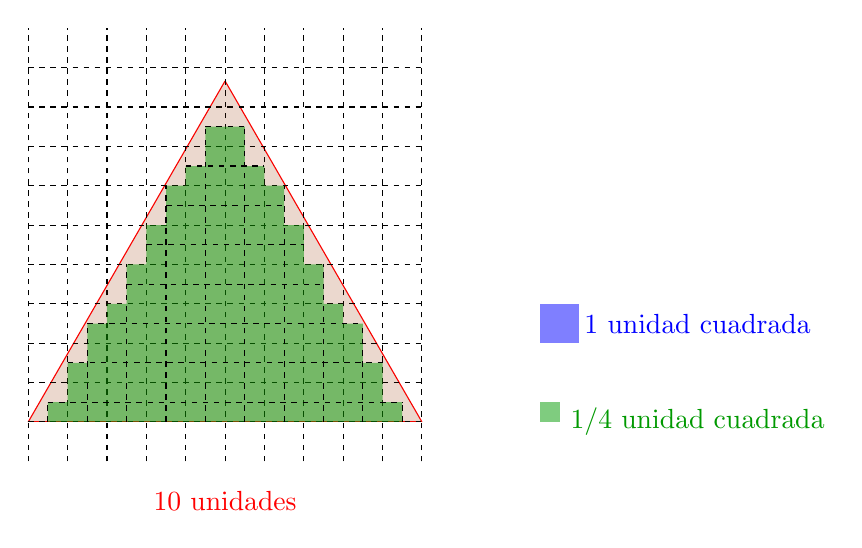
\begin{tikzpicture}[x=0.5cm,y=0.5cm]
\fill[color=zzttqq,fill=zzttqq,fill opacity=0.1] (-5.,0.) -- (5.,0.) -- (0.,8.66025403784) -- cycle;
\draw [color=ffqqqq] (-5.,0.)-- (5.,0.);
\draw [color=ffqqqq] (5.,0.)-- (0.,8.66025403784);
\draw [color=ffqqqq] (0.,8.66025403784)-- (-5.,0.);

\draw [dash pattern=on 2pt off 2pt] (-5,-1) -- (-5,10);
\draw [dash pattern=on 2pt off 2pt] (-4,-1) -- (-4,10);
\draw [dash pattern=on 2pt off 2pt] (-3,-1) -- (-3,10);
\draw [dash pattern=on 2pt off 2pt] (-2,-1) -- (-2,10);
\draw [dash pattern=on 2pt off 2pt] (-1,-1) -- (-1,10);
\draw [dash pattern=on 2pt off 2pt] (0,-1) -- (0,10);
\draw [dash pattern=on 2pt off 2pt] (1,-1) -- (1,10);
\draw [dash pattern=on 2pt off 2pt] (2,-1) -- (2,10);
\draw [dash pattern=on 2pt off 2pt] (3,-1) -- (3,10);
\draw [dash pattern=on 2pt off 2pt] (4,-1) -- (4,10);
\draw [dash pattern=on 2pt off 2pt] (5,-1) -- (5,10);

\draw [dash pattern=on 2pt off 2pt] (-5,0) -- (5,0);
\draw [dash pattern=on 2pt off 2pt] (-5,1) -- (5,1);
\draw [dash pattern=on 2pt off 2pt] (-5,2) -- (5,2);
\draw [dash pattern=on 2pt off 2pt] (-5,3) -- (5,3);
\draw [dash pattern=on 2pt off 2pt] (-5,4) -- (5,4);
\draw [dash pattern=on 2pt off 2pt] (-5,5) -- (5,5);
\draw [dash pattern=on 2pt off 2pt] (-5,6) -- (5,6);
\draw [dash pattern=on 2pt off 2pt] (-5,7) -- (5,7);
\draw [dash pattern=on 2pt off 2pt] (-5,8) -- (5,8);
\draw [dash pattern=on 2pt off 2pt] (-5,9) -- (5,9);
\draw [dash pattern=on 2pt off 2pt] (5,-1) -- (5,10);

\fill[color=zzttqq,fill=zzttqq,fill opacity=0.1] (-5.,0.) -- (5.,0.) -- (0.,8.66025403784) -- cycle;

\fill[color=qqzzqq,fill=qqzzqq,fill opacity=.5] (-4.5,0) -- (-4.5,0.5) -- (-4,0.5) -- (-4,1.5) -- (-3.5,1.5) -- (-3.5,2.5) -- (-3,2.5) -- (-3,3) -- (-2.5,3) -- (-2.5,4) -- (-2,4) -- (-2,5) -- (-1.5,5) -- (-1.5,6) -- (-1,6) -- (-1,6.5) -- (-0.5,6.5) -- (-0.5,7.5) -- (0.5,7.5) -- (0.5,6.5) -- (1,6.5) -- (1,6) -- (1.5,6) -- (1.5,5) -- (2,5) -- (2,4) -- (2.5,4) -- (2.5,3) -- (3,3) -- (3,2.5) -- (3.5,2.5) -- (3.5,1.5) -- (4,1.5) -- (4,0.5) -- (4.5,0.5) -- (4.5,0) -- cycle;
\draw [dash pattern=on 2pt off 2pt] (-4.5,0.5) -- (4.5,0.5);
\draw [dash pattern=on 2pt off 2pt] (-4,1.5) -- (4,1.5);
\draw [dash pattern=on 2pt off 2pt] (-3.5,2.5) -- (3.5,2.5);
\draw [dash pattern=on 2pt off 2pt] (-2.5,3.5) -- (2.5,3.5);
\draw [dash pattern=on 2pt off 2pt] (-2,4.5) -- (2,4.5);
\draw [dash pattern=on 2pt off 2pt] (-1.5,5.5) -- (1.5,5.5);
\draw [dash pattern=on 2pt off 2pt] (-1,6.5) -- (1,6.5);
\draw [dash pattern=on 2pt off 2pt] (-0.5,7.5) -- (0.5,7.5);

\draw [dash pattern=on 2pt off 2pt] (-4.5,0) -- (-4.5,0.5);
\draw [dash pattern=on 2pt off 2pt] (-3.5,0) -- (-3.5,2.5);
\draw [dash pattern=on 2pt off 2pt] (-2.5,0) -- (-2.5,4);
\draw [dash pattern=on 2pt off 2pt] (-1.5,0) -- (-1.5,6);
\draw [dash pattern=on 2pt off 2pt] (-0.5,0) -- (-0.5,7.5);
\draw [dash pattern=on 2pt off 2pt] (0.5,0) -- (0.5,7.5);
\draw [dash pattern=on 2pt off 2pt] (1.5,0) -- (1.5,6);
\draw [dash pattern=on 2pt off 2pt] (2.5,0) -- (2.5,4);
\draw [dash pattern=on 2pt off 2pt] (3.5,0) -- (3.5,2.5);
\draw [dash pattern=on 2pt off 2pt] (4.5,0) -- (4.5,0.5);

\fill[color=qqqqff,fill=qqqqff,fill opacity=0.5] (8,2) -- (9,2) -- (9,3) -- (8,3) -- cycle;
\draw[color=qqqqff] (12,2.5) node {\text{1 unidad cuadrada}};
\fill[color=qqzzqq,fill=qqzzqq,fill opacity=0.5] (8,0) -- (8.5,0) -- (8.5,0.5) -- (8,0.5) -- cycle;
\draw[color=qqzzqq] (12,0) node {\text{1/4 unidad cuadrada}};

\draw[color=ffqqqq] (0,-2) node {\text{10 unidades}};
\end{tikzpicture}
\caption{Cuarto de unidades cuadradas contenidas en el triángulo.}\label{triangulocuartounidaddentro}
\end{center}
\end{figure}



En la figura~\ref{triangulocuartounidadfuera} tenemos los cuadrados de área un cuarto de unidad cuadrada que contienen al triángulo. \\

\begin{figure}[!h]
\begin{center}
\definecolor{ffqqqq}{rgb}{1.,0.,0.}
\definecolor{zzttqq}{rgb}{0.6,0.2,0.}
\definecolor{qqqqff}{rgb}{0.,0.,1.}
\definecolor{ffqqqq}{rgb}{1.,0.,0.}
\definecolor{zzttqq}{rgb}{0.6,0.2,0.}
\definecolor{cqcqcq}{rgb}{0.752941176471,0.752941176471,0.752941176471}
\definecolor{qqzzqq}{rgb}{0.,0.6,0.}

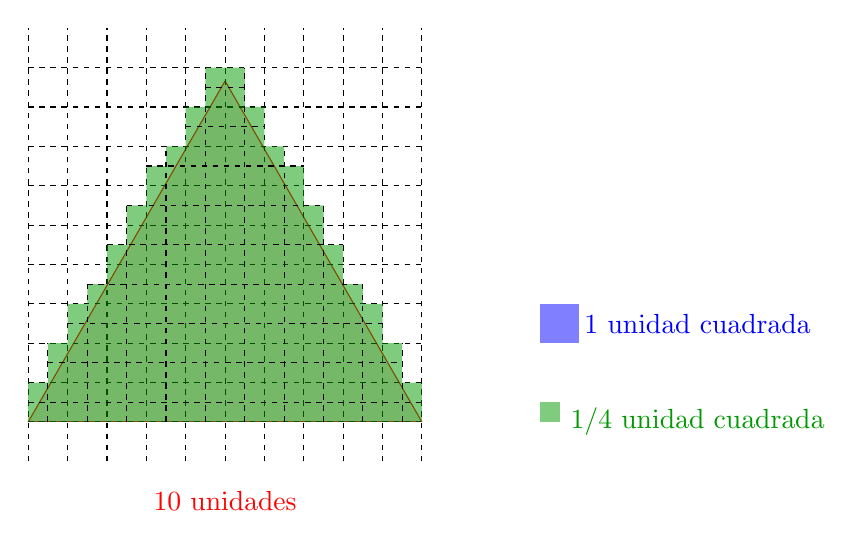
\begin{tikzpicture}[x=0.5cm,y=0.5cm]
\fill[color=zzttqq,fill=zzttqq,fill opacity=0.1] (-5.,0.) -- (5.,0.) -- (0.,8.66025403784) -- cycle;
\draw [color=ffqqqq] (-5.,0.)-- (5.,0.);
\draw [color=ffqqqq] (5.,0.)-- (0.,8.66025403784);
\draw [color=ffqqqq] (0.,8.66025403784)-- (-5.,0.);

\draw [dash pattern=on 2pt off 2pt] (-5,-1) -- (-5,10);
\draw [dash pattern=on 2pt off 2pt] (-4,-1) -- (-4,10);
\draw [dash pattern=on 2pt off 2pt] (-3,-1) -- (-3,10);
\draw [dash pattern=on 2pt off 2pt] (-2,-1) -- (-2,10);
\draw [dash pattern=on 2pt off 2pt] (-1,-1) -- (-1,10);
\draw [dash pattern=on 2pt off 2pt] (0,-1) -- (0,10);
\draw [dash pattern=on 2pt off 2pt] (1,-1) -- (1,10);
\draw [dash pattern=on 2pt off 2pt] (2,-1) -- (2,10);
\draw [dash pattern=on 2pt off 2pt] (3,-1) -- (3,10);
\draw [dash pattern=on 2pt off 2pt] (4,-1) -- (4,10);
\draw [dash pattern=on 2pt off 2pt] (5,-1) -- (5,10);

\draw [dash pattern=on 2pt off 2pt] (-5,0) -- (5,0);
\draw [dash pattern=on 2pt off 2pt] (-5,1) -- (5,1);
\draw [dash pattern=on 2pt off 2pt] (-5,2) -- (5,2);
\draw [dash pattern=on 2pt off 2pt] (-5,3) -- (5,3);
\draw [dash pattern=on 2pt off 2pt] (-5,4) -- (5,4);
\draw [dash pattern=on 2pt off 2pt] (-5,5) -- (5,5);
\draw [dash pattern=on 2pt off 2pt] (-5,6) -- (5,6);
\draw [dash pattern=on 2pt off 2pt] (-5,7) -- (5,7);
\draw [dash pattern=on 2pt off 2pt] (-5,8) -- (5,8);
\draw [dash pattern=on 2pt off 2pt] (-5,9) -- (5,9);
\draw [dash pattern=on 2pt off 2pt] (5,-1) -- (5,10);

\fill[color=zzttqq,fill=zzttqq,fill opacity=0.1] (-5.,0.) -- (5.,0.) -- (0.,8.66025403784) -- cycle;

\fill[color=qqzzqq,fill=qqzzqq,fill opacity=.5] (-5,0) -- (-5,1) -- (-4.5,1) -- (-4.5,2) -- (-4,2) -- (-4,3) -- (-3.5,3) -- (-3.5,3.5) -- (-3,3.5) -- (-3,4.5) -- (-2.5,4.5) -- (-2.5,5.5) -- (-2,5.5) -- (-2,6.5) -- (-1.5,6.5) -- (-1.5,7) -- (-1,7) -- (-1,8) -- (-0.5,8) -- (-0.5,9) -- (0.5,9) -- (0.5,8) -- (1,8) -- (1,7) -- (1.5,7) -- (1.5,6.5) -- (2,6.5) -- (2,5.5) -- (2.5,5.5) --  (2.5,4.5) -- (3,4.5) --(3,3.5) -- (3.5,3.5) --(3.5,3) --  (4,3) -- (4,2) -- (4.5,2) -- (4.5,1) -- (5,1) -- (5,0)-- cycle;

\draw [dash pattern=on 2pt off 2pt] (-5,0.5) -- (5,0.5);
\draw [dash pattern=on 2pt off 2pt] (-4.5,1.5) -- (4.5,1.5);
\draw [dash pattern=on 2pt off 2pt] (-4,2.5) -- (4,2.5);
\draw [dash pattern=on 2pt off 2pt] (-3.5,3.5) -- (3.5,3.5);
\draw [dash pattern=on 2pt off 2pt] (-3,4.5) -- (3,4.5);
\draw [dash pattern=on 2pt off 2pt] (-2.5,5.5) -- (2.5,5.5);
\draw [dash pattern=on 2pt off 2pt] (-2,6.5) -- (2,6.5);
\draw [dash pattern=on 2pt off 2pt] (-1,7.5) -- (1,7.5);
\draw [dash pattern=on 2pt off 2pt] (-0.5,8.5) -- (0.5,8.5);

\draw [dash pattern=on 2pt off 2pt] (-4.5,0) -- (-4.5,2);
\draw [dash pattern=on 2pt off 2pt] (-3.5,0) -- (-3.5,3.5);
\draw [dash pattern=on 2pt off 2pt] (-2.5,0) -- (-2.5,5.5);
\draw [dash pattern=on 2pt off 2pt] (-1.5,0) -- (-1.5,7);
\draw [dash pattern=on 2pt off 2pt] (-0.5,0) -- (-0.5,9);
\draw [dash pattern=on 2pt off 2pt] (0.5,0) -- (0.5,9);
\draw [dash pattern=on 2pt off 2pt] (1.5,0) -- (1.5,7);
\draw [dash pattern=on 2pt off 2pt] (2.5,0) -- (2.5,5.5);
\draw [dash pattern=on 2pt off 2pt] (3.5,0) -- (3.5,3.5);
\draw [dash pattern=on 2pt off 2pt] (4.5,0) -- (4.5,2);

\fill[color=qqqqff,fill=qqqqff,fill opacity=0.5] (8,2) -- (9,2) -- (9,3) -- (8,3) -- cycle;
\draw[color=qqqqff] (12,2.5) node {\text{1 unidad cuadrada}};
\fill[color=qqzzqq,fill=qqzzqq,fill opacity=0.5] (8,0) -- (8.5,0) -- (8.5,0.5) -- (8,0.5) -- cycle;
\draw[color=qqzzqq] (12,0) node {\text{1/4 unidad cuadrada}};

\draw[color=ffqqqq] (0,-2) node {\text{10 unidades}};
\end{tikzpicture}
\caption{Cuarto de unidades cuadradas que contienen al triángulo.}\label{triangulocuartounidadfuera}
\end{center}
\end{figure}

Así, podemos mejorar nuestra aproximación como sigue:

$$ 146 \cdot \frac{u^2}{4}< \text{área del triángulo} < 200 \cdot \frac{u^2}{4}$$

es decir, tenemos

$$ 36 u^2 + 2\cdot \frac{u^2}{4}< \text{área del triángulo} < 50 u^2$$

¡Nos hemos aproximado más a nuestro objetivo!
\end{pba}

Con este procedimiento, podemos determinar el área del triángulo equilátero de lado 10 unidades y de cualquier polígono que se nos presente con cualquier longitud en cada lado: rectángulos, triángulos rectángulos, rombos, pentágonos regulares, pentágonos irregulares, etcétera. \\

De hecho, podemos determinar el área de cualquier figura con este procedimiento (¡aunque no sea un subconjunto del plano!).\\


%%%%%%%%%
%%%%%%%%% CAMBIAR TRIÁNGULO POR CUADRADO DE LADOS RACIONALES
%%%%%%%%%


Nosotros nos enfocaremos a tratar de determinar el área de algunos subconjuntos específicos del plano: los triángulos.

\begin{obs}
El área de cualquier objeto siempre es un número real no negativo.
\end{obs}
\begin{obs}\label{ob2}
Si $\square ABCD$ es un rectángulo, el $\A(\square ABCD)= |AB||BC|$.
\end{obs}

\begin{df}
Diremos que $\triangle ABC$ es un \textcolor{red}{\bf triángulo rectángulo}\index{triángulo ! rectángulo} si uno de sus ángulos internos es $\perp$.
\end{df}

Ya estamos muy cerca de nuestro objetivo, antes de ello probaremos la siguiente proposición:

\begin{prop}\label{prop1}
Sea $ \triangle ABC$ un triángulo rectángulo tal que $|\angle CBA|= \perp $ entonces el $\A(\triangle ABC)= \frac{|AB||BC|}{2}$.
\end{prop}

\begin{pba}
Sean $l$ la recta paralela a $\overline{AB}$ por $C$, $m$ la recta paralela a $\overline{BC}$ por $A$ y $l \cap m$=$\{D\}$. Consideremos al rectángulo $\square ABCD$ (¿realmente es un rectángulo?, ver sección de ejercicios: Ejercicio~\ref{rectángulo}) y una diagonal que en este caso, sin pérdida de generalidad, elegiremos a $AC$. Entonces $\triangle ABC \equiv \triangle CDA$ \textbf{cc(ALA)} ya que comparten el lado $AC$ y como $l$ y $\overline{AB}$ son paralelas y $\overline{AC}$ es una recta transversal, se cumple que $|\angle CAD|=|\angle ACB|$ y $|\angle DCA|=|\angle BAC|$.
Ahora, notemos que si dos triángulos son congruentes, entonces su área es la misma\footnote{Dados $\triangle ABC$ y $\triangle DEF$ tales que $\triangle ABC \equiv \triangle DEF$, por la Definición~\ref{dfárea}, tenemos que si $\A(\triangle ABC)=\alpha$, entonces caben $\alpha$ unidades cuadradas en $\triangle ABC$, ahora como $\triangle ABC \equiv \triangle DEF$ la magnitud de los lados del $\triangle DEF$ es la misma que la de los lados del $\triangle ABC$ así que tanbién caben $\alpha$ unidades cuadradas en $\triangle DEF$ y por tanto tienen la misma área.}.
%%%
%%% triángulos congruentes tienen la misma área 
%%% REALIZADO :)
%%% VERIFICAR UNICIDAD DE LA PARALELA  (GASDE)

Así, tenemos que:
\begin{eqnarray*}
\A (\square ABCD) &=& \A (\triangle ABC)+\A(\triangle CDA)\\
&=&\A (\triangle ABC)+\A(\triangle ABC)\\
&=&2\cdot \A(\triangle ABC)
\end{eqnarray*}

Y, por la Observación~\ref{ob2}, se sigue que: $|AB||BC|= 2 \cdot \A (\triangle ABC)$.

Por lo tanto,
$$\A(\triangle ABC)=\frac{|AB||BC|}{2}$$
\end{pba}

\begin{df}\label{ADUT}
Sean $\triangle ABC$ y $X \in \{A, B, C\}$.

$h_{X}$ es la \textcolor{red}{{\bf altura por el vértice X}}\index{altura de un triángulo} si y solamente si $h_{X}$ es la recta ortogonal por $X$ a la recta determinada por $\{A, B, C\} \setminus \{X\}$. A la intersección de $h_{X}$ con la recta determinada por $\{A, B, C\} \setminus \{X\}$ se le llama \textcolor{red}{\bf pie de la altura por X}\index{pie de altura}.
\end{df}

Es decir, consideremos $\triangle ABC$, entonces tenemos lo siguiente:
\begin{itemize}
\item $h_{A}$ es la recta ortogonal al lado $BC$ por el vértice $A$ y sea $h_{A}\cap BC=\{D\}$.
\item $h_{B}$ es la recta ortogonal al lado $CA$ por el vértice $B$ y sea $h_{B}\cap CA=\{E\}$.
\item $h_{C}$ es la recta ortogonal al lado $AB$ por el vértice $C$ y sea $h_{C}\cap AB=\{F\}$.
\end{itemize}
De esta manera, se tiene que $D$, $E$ y $F$ son los pies de altura por $A$, $B$ y $C$ respectivamente.
%%%%%
%%%%% Ejemplos y notación de los pies de las alturas
%%%%% REALIZADO :)

\begin{prop} \label{prop2}
Sea $\triangle ABC$ y $X \in \{A,B,C\}$. Si $D$ es el pie de la altura por $A$, $E$ es el pie de la altura por $B$ y $F$ es el pie de la altura por $C$ entonces
$$\A(\triangle ABC) = \frac{|BC||AD|}{2}= \frac{|CA||BE|}{2} = \frac{|AB||CF|}{2} $$
\end{prop}

\begin{pba}
Daremos una prueba de la primer igualdad que no dependerá de la elección de los vértices, por lo que la misma prueba servirá para probar las otras dos igualdades (ver sección de ejercicios, Ejercicio~\ref{area}).

Haremos la prueba para $X=A$. Sea $h_A \cap \overline{BC} =\{D\}$. Notemos que tenemos tres casos:
\begin{enumerate}
\item $\frac{BD}{DC} < 0$. 
\begin{enumerate}
\item Supongamos que $0 < \frac{DB}{BC}$.

Consideremos a los triángulos $\triangle ADC$ y $\triangle ADB$. Notemos que ambos triángulos son rectángulos (pues $\overline{AD}$ es ortogonal a $\overline{BC}$) por lo que, debido a la Proposición~\ref{prop1}, se tiene que
$$\A(\triangle ADC)= \frac{|DC||AD|}{2} \quad \text{y} \quad \A(\triangle ADB) = \frac{|DB||AD|}{2}$$

Puesto que $\triangle ABC$ está contenido en $\triangle ADC$ tenemos que
\begin{eqnarray*}
\A(\triangle ABC) &=& \A(\triangle ADC)-\A(\triangle ADB)\\
&=& \frac{|DC||AD|}{2} -  \frac{|DB||AD|}{2}\\
&=& \left(|DC|-|DB|\right)\frac{|AD|}{2} 
\end{eqnarray*}

Por hipótesis, $\frac{BD}{DC}<0$ y $0< \frac{DB}{BC}$, por lo que
\begin{itemize}
\item $0<BD \Rightarrow DC<0$ y $BC <0$. Así,
\begin{eqnarray*}
\A(\triangle ABC) &=& \left(|DC|-|DB|\right)\frac{|AD|}{2}\\
&=&   \left(CD-(-DB)\right)\frac{|AD|}{2}\\
&=&   \left(CD +DB\right)\frac{|AD|}{2} = \frac{(CB)|AD|}{2} \\
&=& \frac{|BC||AD|}{2}\\
\end{eqnarray*}


%%%
%%%
%%%

\item $BD<0 \Rightarrow 0<DC$ y $0<BC$. Así, 
\begin{eqnarray*}
\A(\triangle ABC) &=& \left(|DC|-|DB|\right)\frac{|AD|}{2}\\
&=&   \left(DC-DB\right)\frac{|AD|}{2}\\
&=&   \left(DC+(-DB)\right)\frac{|AD|}{2}\\
&=&   \left(DC+BD\right)\frac{|AD|}{2}\\
&=&   \left(BD+DC\right)\frac{|AD|}{2}\\
&=& \frac{(BC)|AD|}{2}=\frac{|BC||AD|}{2}\\
\end{eqnarray*}
\end{itemize}

%%%
%%%REALIZADO
%%% :)
		 

\item Si $0 <\frac{BC}{CD}$ la prueba es análoga (ver sección de ejercicios, Ejercicio~\ref{cortafuera}).		 

\end{enumerate}

\item $0= \frac{BD}{DC}$

En este caso, estamos diciendo que $B=D$, por lo que $\overline{AB}$ es ortogonal a $\overline{BC}$; es decir, $\triangle ABC$ es un triángulo rectángulo y podemos hacer uso de la Proposición~\ref{prop1}.

\item $0< \frac{BD}{DC}$.

%%%
%%%
%%%

Consideremos los triángulos $\triangle ABD$ y $\triangle ADC$, notemos que ambos triángulos son rectángulos ya que AD es ortogonal a BC, entonces por la Proposición \ref{prop1} el $\A(\triangle ABD)$= $\frac{|BD||AD|}{2}$ y el $\A(\triangle ADC)$= $\frac{|DC||AD|}{2}$ así que como	el $\A(\triangle ABC)$=$\A(\triangle ABD)$+$\A(\triangle ADC)$ se tiene que:
		 
$\A(\triangle ABC)$=$\frac{|BD||AD|}{2}$ +  $\frac{|DC||AD|}{2}$= $\frac{|AD|(|BD|+|DC|)}{2}$=$\frac{|AD||BC|}{2}.$
		
Veamos como en el primer caso que el resultado no depende de la orientación de los segmentos. 
Por hipótesis $0< \frac{BD}{DC}$, entonces:
\begin{enumerate}
\item Si $0<BD \Rightarrow 0<DC.$
\begin{itemize}
\item Si $0<AD$, entonces:
\begin{eqnarray*}
\A(\triangle ABC)
&=&  \frac{|BD||AD|}{2} + \frac{|DC||AD|}{2}\\
&=&  \frac{(BD)(AD)}{2} + \frac{(DC)(AD)}{2}\\
&=&  \frac{(AD)(BD+DC)}{2}=\frac{(AD)(BC)}{2}\\
&=&  \frac{|AD||BC|}{2}.\\ 
\end{eqnarray*}
\item Si $AD<0$, entonces:
\begin{eqnarray*}
\A(\triangle ABC)
&=&  \frac{|BD||AD|}{2} + \frac{|DC||AD|}{2}\\
&=&  \frac{(BD)(DA)}{2} + \frac{(DC)(DA)}{2}\\
&=&  \frac{(DA)(BD+DC)}{2}=\frac{(DA)(BC)}{2}\\
&=&  \frac{|AD||BC|}{2}.\\ 
\end{eqnarray*}		
\end{itemize}		 
\item Si $BD<0 \Rightarrow DC<0$
\begin{itemize}
\item Si $0<AD$, entonces:
\begin{eqnarray*}
\A(\triangle ABC)
&=&  \frac{|BD||AD|}{2} + \frac{|DC||AD|}{2}\\
&=&  \frac{(DB)(AD)}{2} + \frac{(CD)(AD)}{2}\\
&=&  \frac{(AD)(DB+CD)}{2}=\frac{(AD)(CD+DB)}{2}\\
&=&  \frac{(AD)(CB)}{2}=\frac{|AD||BC|}{2}.\\ 
\end{eqnarray*}
\item Si $AD<0$, entonces:
\begin{eqnarray*}
\A(\triangle ABC)
&=&  \frac{|BD||AD|}{2} + \frac{|DC||AD|}{2}\\
&=&  \frac{(DB)(DA)}{2} + \frac{(CD)(DA)}{2}\\
&=&  \frac{(DA)(DB+CD)}{2}=\frac{(DA)(CD+DB)}{2}\\
&=&  \frac{(DA)(CB)}{2}=\frac{|AD||BC|}{2}.\\ 
\end{eqnarray*}		
\end{itemize}
\end{enumerate}
\end{enumerate}
	
\end{pba}


%%%% Hacer los subcasos
%%% CORRECCIÓN REALIZADA :)
%%%%DUDA: CASO 2 (REVISAR) 


%%%%%% Cuidar la longitud de la altura :)
Así, la proposición Proposición~\ref{prop2} nos da la forma de calcular el área de cualquier triángulo dado. 
Enseguida, se mencionan un par de resultados que relacionan el área de dos triángulos. 
		 
\begin{prop}\label{prop3}
Sean $\triangle ABC$ y $\triangle DEF$ tales que $|AB|=|DE|$ y consideremos $h_{C}\cap AB=\{G\}$ y $h_{F}\cap DE=\{H\}$, entonces:
$$\frac{\A(\triangle ABC)}{\A(\triangle DEF)}= \frac{|CG|}{|FH|}.$$
		
\end{prop}
\begin{pba} Por la Proposición~\ref{prop2}, tenemos que:
$$\frac{\A(\triangle ABC)}{\A(\triangle DEF)}= \frac{\frac{|CG||AB|}{2}}{\frac{|FH||DE|}{2}}$$
Como $|AB|=|DE|$, concluimos que:
$$\frac{\A(\triangle ABC)}{\A(\triangle DEF)}= \frac{|CG|}{|FH|}$$
\end{pba}
		 
\begin{prop}\label{prop4}
Sean $\triangle ABC$ y $\triangle DEF$ y consideremos $h_{C}\cap AB=\{G\}$ y $h_{F}\cap DE=\{H\}$, tales que $|CG|=|FH|$, entonces: 
$$\frac{\A(\triangle ABC)}{\A(\triangle DEF)}= \frac{|AB|}{|DE|}.$$
\end{prop}
\begin{pba}Por la Proposición~\ref{prop2}, tenemos que:
$$\frac{\A(\triangle ABC)}{\A(\triangle DEF)}= \frac{\frac{|CG||AB|}{2}}{\frac{|FH||DE|}{2}}$$ 
Como $|CG|=|FH|$ se sigue que:
$$\frac{\A(\triangle ABC)}{\A(\triangle DEF)}= \frac{|AB|}{|DE|}$$
\end{pba}
 
%%%%%%%
%%%%%%%Notación en las pruebas anteriores
%%%%%%%CORRECCIÓN REALIZADA :) 


\subsection*{Ejercicios}

\begin{enumerate}

\item Demostrar que si  $\square ABCD$ es un paralelogramo tal que un ángulo interno es recto entonces todos sus ángulos internos son rectos.

\item  Demostrar que si $\square ABCD$ es un cuadrado tal que $|AB|=\alpha \in \N$ entonces $\A(\square ABCD)=\alpha^{2}$.

\item Demostrar que, en la Proposición~\ref{prop1} (página \pageref{prop1}), la construcción dada forma efectivamente un rectángulo.\label{rectángulo}

\item En la Proposición~\ref{prop2} (página \pageref{prop2}), probar el  caso en el que $0<\frac{BC}{CD}$.\label{cortafuera}

\item Verificar que la prueba de la Proposición~\ref{prop2} (página \pageref{prop2}) no depende de la elección de los vértices. (Sugerencia: Sigue la misma prueba solamente cambiando de vértices y del respectivo pie de altura).\label{area}
\end{enumerate}


